%!TEX root = ..\MainFile.tex
\chapter{Групповые явления в жизни животных} % (fold)
\label{cha:NatureFlocking}

\epigraph{Если сто бегунов как один бегут,\\
Это можно назвать так и сяк.\\
У лошадей это будет табун,\\
У рыб это будет косяк.}{Машина Времени}

\section{Методы наблюдения и сбора информации} % (fold)
\label{sec:ExperimentalMethods}
	Главная сложность в выполнении экспериментального наблюдения за группой животных или, тем более, насекомых заключается в трудности отслеживания траекторий отдельных особей. Это связано с тем, что рассматриваемые колонии или группы
	\begin{itemize}
		\item  состоят из множества индивидов, которые
		\item выглядят очень похоже
		\item и в основном очень быстро перемещаются
	\end{itemize}
	Кроме того, необходимо учитывать крайнее разнообразие живых организмов, за перемещением которых необходимо наблюдать, поскольку, как уже говорилось во введении, изменение поведения при обьединении в группы наблюдается для широкого разнообразия типоразмеров животных --- начиная от бактерий в пробирке~\cite{csahok1997,keller1971} и заканчивая китами на океанских просторах~\cite{makris2009}.
	Несмотря на совсем неочевидные методы решения этих проблем, изучению группового поведения на протяжении многих лет посвящалось значительное внимание.

	Условно их можно разделить на две неравные группы: в одну отнесем так или иначе методы с использованием визуальных средства (т.е. фото- и видеокамер в комбинации с различного рода маячками или метками), а в другую --- сравнительно недавно начавшие применяться методы с использованием GPS-систем.

	Классическим может считаться метод измерения скорости по изображениям частиц~\cite{raffel2007}. Обычно он применяется для измерения скорости потока жидкости или газа: в исследуемую среду вводится краситель, состоящий из броуновских частиц, и при помощи наблюдения за перемещением этого вещества возможно определить линии тока в исследуемой среде. Применимо к самодвижущимся частицам метод успешно был применен Czir\'{o}k  et all\cite{csahok1997}, которые при помощи фазово-контрастной микроскопии исследовали групповое движение молекул.

	Когда речь заходит об исследовании стай птиц (стад животных), размер индивидов больше, однако, в отличие от бактерий, область перемещения слабо ограничена. Чтобы обойти эту сложность, например, Becco et all~\cite{becco2006} ограничили движение рыб по высоте, используя плоский аквариум.

	Использование нескольких камер для съемки стай с разных точек в дальнейшем требовало трудоемкой обработки результатов для получения трехмерной картины, но позволило получить мгновенные снимки положения сотен скворцов в стае~\cite{ballerini2008}, однако получить траектории движения не удалось.

	По мере развития технологий стало возможным создать маячки GPS --- достаточно маленькие, чтобы их можно было закрепить на животном или птице, не мешая ему. Ограничением такого подхода является возрастающая стоимость исследования. Были проведены исследования пар~\cite{biro2006,nagy2010} или даже шестерок~\cite{dellariccia2008} тренированных голубей.

	Помимо вышесказанного, в настоящее время увеличение точности сонаров и разработка определенной технологии применения, в которой океан выступает в роли акустического волновода, позволило использовать их для единовременного наблюдения за огромными количествами рыб на больших территориях океанического шельфа.~\cite{makris2006}

	Подводя итоги, можно отметить увеличение роли комьютера в накоплении и обработке экспериментальных данных. Текущая динамика позволяет надеяться, что со временем будут получены данные не меньшей точности, чем получаемые во время численных экспериментов по различным моделям.
% subsection subsection_name (end)
\section{Основные результаты наблюдений} % (fold)
\label{sec:ObservationResults}
	Поскольку экспериментальное наблюдение стадных явлений не является темой данной работы, мы не будем останавливаться подробно на результатах полевых или лабораторных исследованиях, тем более что всестороннее освещение этого вопроса дано в работе Вичека~\cite{vicsek2012}. Однако для лучшего понимания распространенности в природе стадных явлений будет приведен краткий обзор наиболее характерных, с нашей точки зрения, работ, сгруппированных по исследуемому материалу. Итак, в разные годы обьектами исследования становились:
	\begin{enumerate}
		\item Внутриклеточные соединения~\cite{chowdhury2006,keller1971}
		\item Колонии бактерий~\cite{czirok1998,csahok1997}
		\item Насекомые~\cite{buhl2006}
		\item Птицы~\cite{ballerini2008,selous1931,dellariccia2008,biro2006,major1978,nagy2010}
		\item Рыбы~\cite{cambui2012,makris2009,parrish1997}
		\item Млекопитающие, к примеру, буйволы~\cite{sinclair1977}
	\end{enumerate}
	Особняком в этом ряду стоят наблюдения за океаническим планктоном~\cite{seuront2004} и превышающие по своей численности наблюдения за любым другим типом обьектов, наблюдения за поведением групп людей, например~\cite{parisi2009,moussaid2011}.%ссылка про транспортные потоки

	Кроме того, в совершенно отдельную группу необходимо выделить лабораторные эксперименты, проводимые с неживыми обьектами --- нематической жидкостью, колеблющимися металлическими стержнями, наночастицами в жидкости, микророботами и тому подобным.~\cite{schaller2010,turgut2008,blair2003}

	Теперь приведем основные результаты, полученные в ходе наблюдений. Для начала, необходимо четко разделять работы, в которых исследования велись на плоскости (все, кроме указанных далее) и в которых наблюдения велись в трехмерном пространстве~\cite{cullen1965,ballerini2008,major1978,makris2009}. Хотя, как выяснилось, для рыб такое разделение не вполне необходимо. Но обо всем по порядку.

	Главный вывод, который в общем-то и не нуждается в подтверждении --- это то, что существует отдельный класс перемещений группы индивидов как целого, и при этом перемещения отдельных индивидов оказываются упорядочены. То есть, при определенных условиях (чаще всего рассматривается различная плотность на единицу площади, или обеспеченность ресурсами в широком смысле слова) происходит спонтанное нарушение симметрии, и хаотическое движение сменяется упорядоченным. Как уже говорилось, это наблюдается на всех масштабах природы, и более того --- совершенно не обязательно при этом прямое (визуальное или тактильное) взаимодействие между особями, и бывает достаточно опосредствованного взаимодействия через среду обитания~\cite[с. 119]{vicsek2012}. %добавить информацию про молекулы, перекидывающие взаимодействие через жидкость в которой они живут
	Следующее наблюдение на которое указывают многие авторы: при нарушении симметрии возникает и дальний порядок связи, к примеру, рыбы могут изменять общее направление движения практически мгновенно~\cite{cambui2012}, а птицы --- так-же быстро принимать решения о посадке.~\cite{lukeman2010,major1978}.

	более того, самым удивительным явлется то, что у всех живых существ и неживых предметов, при движении которых проявляются стадные явления, качественный характер этих явлений практически одинаков. %(Не считая сугубо трехмерных формаций, которые образуются в стаях птиц, однако и там можно выделить правильный ``параметр порядка'').
	\begin{figure}
        \centering
        \begin{subfigure}{.4\columnwidth}
                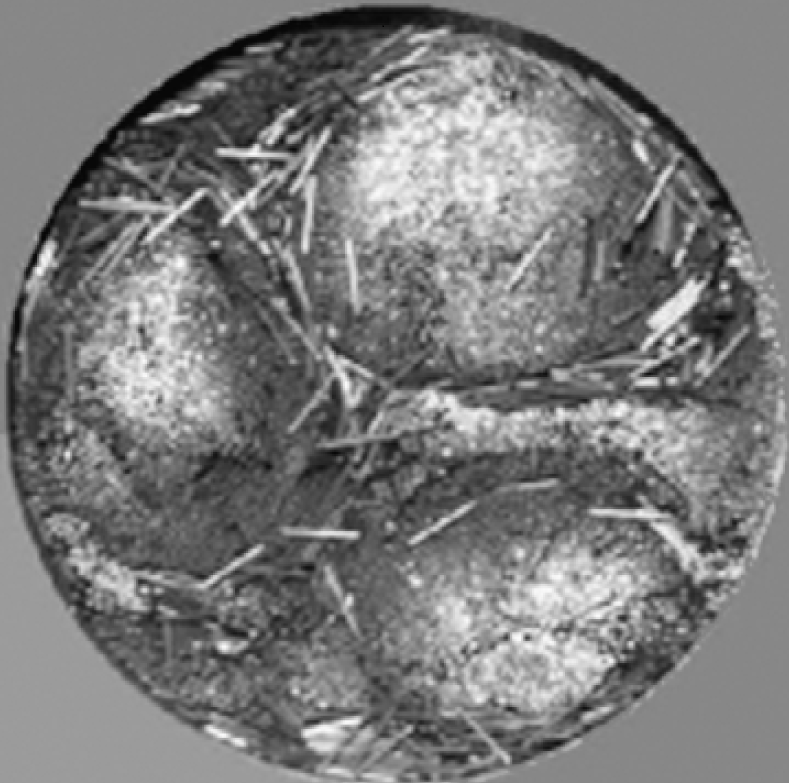
\includegraphics[width=\columnwidth]{Images/Fig4_CollectiveMotion.png}
                \caption{A nematics}
                \label{fig:CollMot:nematics}
        \end{subfigure}%
        ~ %add desired spacing between images, e. g. ~, \quad, \qquad, \hfill etc.
          %(or a blank line to force the subfigure onto a new line)
        \begin{subfigure}{.4\columnwidth}
                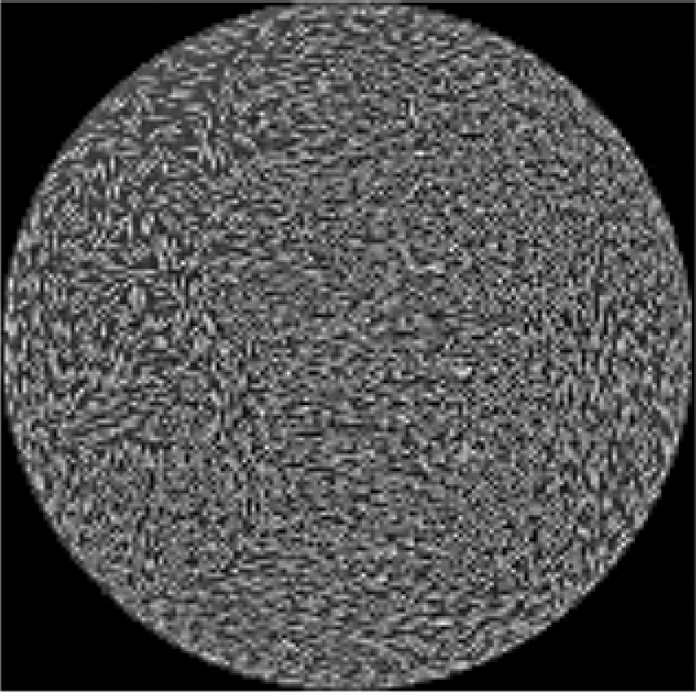
\includegraphics[width=\columnwidth]{Images/Fig6_CollectiveMotion}
                \caption{A rods on wibe}
                \label{fig:CollMot:rods}
        \end{subfigure}
        \caption{Упорядочивание неживых обьектов}
        \label{fig:CollMot:NonLiving}
    \end{figure}
        ~ %add desired spacing between images, e. g. ~, \quad, \qquad, \hfill etc.
          %(or a blank line to force the subfigure onto a new line)
    \begin{figure}
    	\centering
        \begin{subfigure}{0.3\textwidth}
                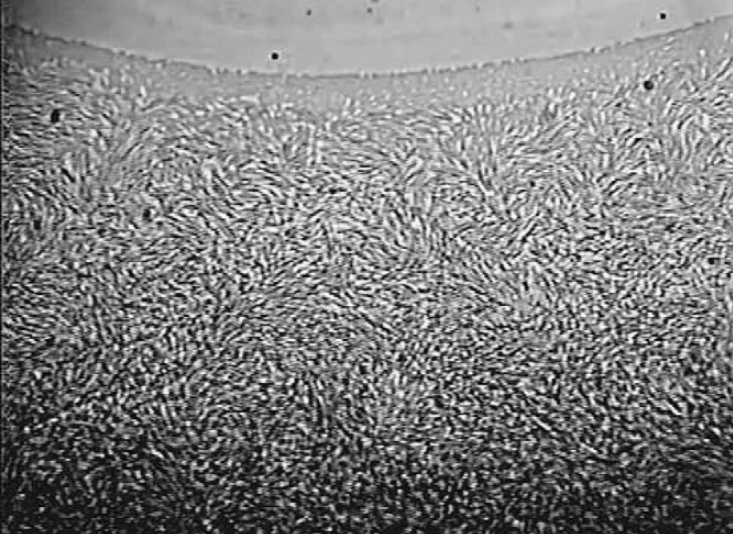
\includegraphics[width=\textwidth]{Images/Fig11_CollectiveMotion}
                \caption{A bacteria 1}
                \label{fig:CollMot:bacteria}
        \end{subfigure}
        \begin{subfigure}{0.5\textwidth}
                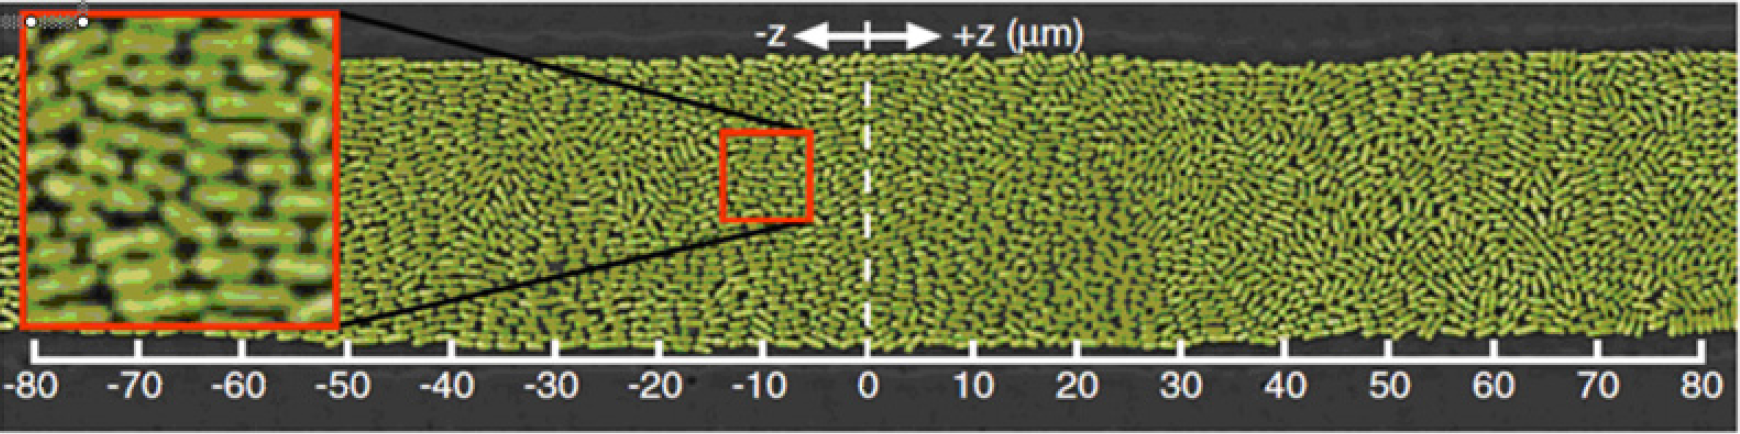
\includegraphics[width=\textwidth]{Images/Fig15_CollectiveMotion_part}
                \caption{A moleculae}
                \label{fig:CollMot:moleculae}
        \end{subfigure}
        \caption{Микроскопические проявления групповой динамики}
        \label{fig:CollMot:microscpoic}
    \end{figure}
    \begin{figure}
    	\centering
        \begin{subfigure}{0.4\textwidth}
                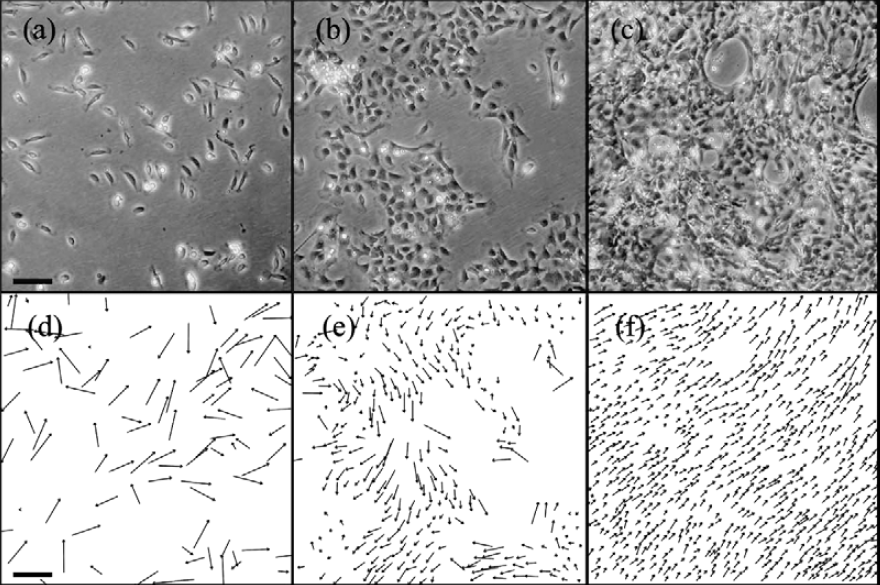
\includegraphics[width=\textwidth]{Images/Fig17_CollectiveMotion}
                \caption{A fishes}
                \label{fig:CollMot:fishes}
        \end{subfigure}
        \begin{subfigure}{0.4\textwidth}
                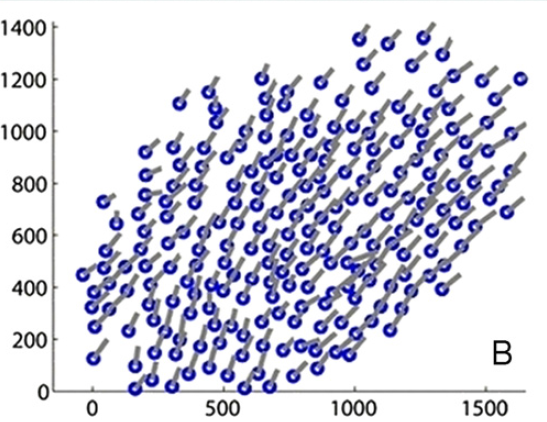
\includegraphics[width=\textwidth]{Images/Fig29_CollectiveMotion_part}
                \caption{A ducks}
                \label{fig:CollMot:ducks}
        \end{subfigure}
        \caption{Макроскопические проявления группового движения}\label{fig:CollMot:macroscopic}
	\end{figure}

	Наглядно это можно рассмотреть на рис. \ref{fig:CollMot:NonLiving}, \ref{fig:CollMot:microscpoic}, \ref{fig:CollMot:macroscopic}. Особенностью всех представленных на изображениях обьединений является то, что они расположены на плоскости. И, как мы видим, возникает два типа упорядоченностей, иногда (как на рис. \ref{fig:CollMot:nematics}) проявляющихся единовременно: это упорядоченное движение в спонтанно выбранном направлении или упорядоченное обращение вокруг некоторого центра. Видно также, что для совершенно, казалось бы, различных обьектов групповое поведение является очень схожим.

	Что же касается перемещений, не ограниченных в двух плоскостях, то нам хотелось бы заострить внимание на трех моментах. 

	Во-первых, в обьемном пространстве также наблюдаются все вышеперечисленные упорядоченные перемещения: птицы сбиваются в стаю и летят в выбранном направлении~\cite{dellariccia2008}, насекомые кружат вокруг улья~\cite{buhl2006} и т.п.

	\begin{wrapfigure}{r}{0.5\textwidth}
	  \vspace{-20pt}
	  \begin{center}
	    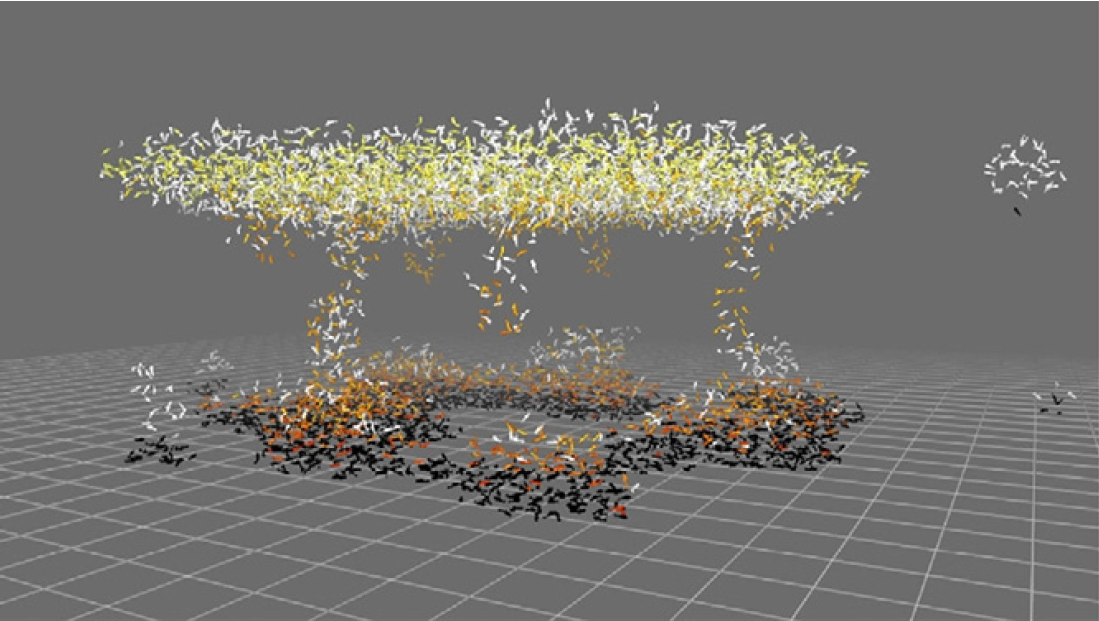
\includegraphics[width=0.48\textwidth]{Images/Fig57_CollectiveMotion}
	  \end{center}
	  \vspace{-20pt}
	  \caption{Расслоение косяка рыб}
	  \label{fig:FishSplitting}
	  \vspace{-10pt}
	\end{wrapfigure}

	Во-вторых, и это является особенностью косяков рыб, возможно расслоение трехмерной группы на более плоские подгруппы, с наличием соединяющих (цилиндрических) столбов. Предполагается, что это это связано с ``мотивацией'', например, молодая стерлядь во время нереста предпочитает подниматься выше, а более старая опускается вниз.~\cite{axelsen2000} При этом наблюдаются структуры подобные изображенным на рис. \ref{fig:FishSplitting}

    \begin{figure}
    	\centering
        \begin{subfigure}{0.4\textwidth}
            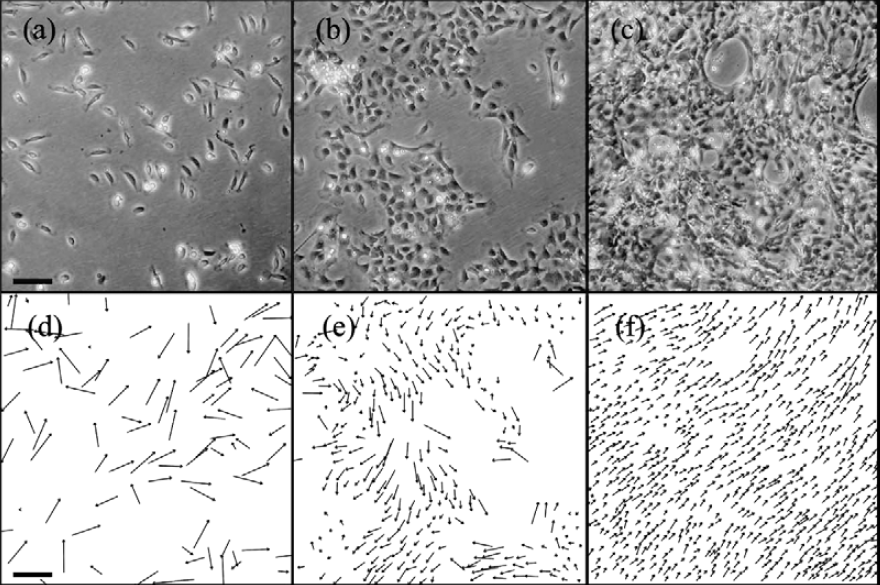
\includegraphics[width=\textwidth]{Images/Fig17_CollectiveMotion}
            \caption{A fishes}
            \label{fig:CollMot:Birds}
        \end{subfigure}
        \begin{subfigure}{0.4\textwidth}
            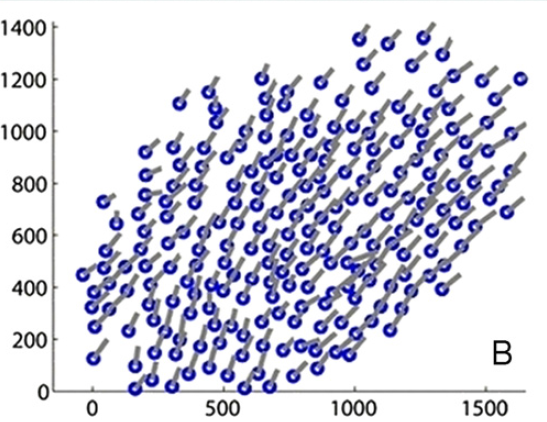
\includegraphics[width=\textwidth]{Images/Fig29_CollectiveMotion_part}
            \caption{A ducks}
            \label{fig:CollMot:Plancton}
        \end{subfigure}
    \caption{Макроскопические проявления группового движения []}
    \label{fig:CollMot:Volumetric}
	\end{figure}

	\marginpar{}
    И в-третьих, поскольку основное внимание при наблюдениях в трехмерном пространстве уделялось птицам и рыбам, групповая динамика которых хоть и обладает большим количеством подобных черт, все же разнятся в том что стаи птиц не расслаиваются по высоте, тем более ярко проявляется аналогия между пространственными формированиями птиц и морского планктона []
    \marginpar{необходимо уточнить что имелось ввиду в~\cite{seuront2004}}%уточнить!!!!
	
    \textcolor{red}{В дальнейшем в этой части можно указать что в групповых явлениях наблюдаются ``лидеры'', которые могут задавать движение. Еще где-то надо сказать что фазовый переход переходит или при уменьшении шума, или при увеличении плотности, наверно в следующем пункте}

% subsection основные_результаты_наблюдений_за_системами_демонстрирующими_группувую_динамику (end)
\section{Количественные характеристики группового движения} % (fold)
\label{sec:NumericalCharacteristicsCollMot}
    Не смотря на то, что подобность движений различных типов обьектов очевидна, для какого-либо исследования нельзя обойтись без количественных характеристик явления.
    Укажем отдельно характеристики обьектов, которые участвуют в коллективном движении:
    \begin{enumerate}
        \item все они похожи друг на друга
        \item они перемещаются с почти постоянной скоростью и способны изменять направление движения
        \item При сближении, взаимодействие приводит к выравниванию направления движения
        \item Выравнивание происходит с ошибками (шумом)
    \end{enumerate}

    Для совокупности обьектов, характерным является наличие фазового перехода от разупорядоченного движения к упорядоченному.

    Помня о том, что изменяется только направление движения каждого обьекта, в качестве параметра порядка было естественно определить следующую величину:
    \begin{equation}\label{eq:OrederParam}
        \varphi = \frac{1}{N v_0} |{\sum\limits_{i=1}^n \vec{v}_i}|
    \end{equation}
    Тогда мерой упорядоченности системы является модуль средней скорости, нормированной на единицу. В уравнении \ref{eq:OrederParam} $N$ --- полное число обьектов, $v_0$ --- средний модуль скорости обьектов в системе. Понятно, что если движение неупорядочено, то скорости обьектов направлены случайным образом, и такая сумма будет стремиться к нулю. Если же скорости направлены вдоль некоторого выбранного направления, то параметр порядка стремится к единице. Разумеется, как и всяческий статистический параметр, выражаемый через средние величины, это выражение имеет смысл только при больших $N$, иначе величина флуктуаций из-за кадого обьекта будет слишком высокой.

    Из статистической физики нам известно, что фазовый переход может происходить как в равновесной (замкнутой), так и в неравновесной системе. Ввиду того что в групповом движении, согласно рассматриваемой модели, участвуют самодвижущиеся частицы становится понятно, что системы с групповой динамикой сугубо неравновесны. Неравновесная статистическая физика в последнее десятилетие выделилась в отдельное направление физики, со своим словарем, обьектом исследований и характерными процессами, вызывающими наибольший интерес исследователей в текущий момент времени. И потому, возможно, было бы предпочтительнее модифицировать модель или провести аналогии с фазовыми переходами, рассматриваемыми в рамках равновесной статистической физики.~\cite{vicsek2012}

    Эта идея, однако, кажется не приемлимой по нескольким соображениям: во-первых, в системах, демонстрирующих групповую динамику, наблюдаются совершенно не характерные для равновесной термодинамики явления, такие как ``пробки'' или флуктуации гигантского числа частиц. А во-вторых, статистическая механика имеет дело с количеством частиц, стремящимся к бесконечности ($10^{23}$), и в рамках этого допущения определяет остальные понятия, в то время как явления группового перемещения наблюдаются при числе частиц, редко превышающем десятки тысяч.

    Интересным было замечание \cite{tu2000}, указывающее на значительную аналогию в поведении систем, демонстрирующих групповую динамику, и феромагнитных систем. К примеру, рассматривая критические экспоненты, связанные с параметром порядяка вида:
    \begin{equation}
        \sigma \sim |1-\eta/\eta_c|^{-\gamma}
    \end{equation}
    позволяют вычислить критические индексы $\gamma$. При этом получается, что критические индексы вычисленные, скажем, по модели Изинга, и вычисленные из (численных) экспериментов с системами, демонстрирующими групповую динамику, оказываются в хорошем согласии между собой.

    Итак, резюмируя, в системах с коллективными эффектами происходит фазовый переход, при этом параметром порядка выступает средняя векторная скорость \ref{eq:OrederParam}, а в качестве ``температуры'' --- шум, т.е. некоторое добавочное воздействие, которое случайным образом изменяет направление движения каждого обьекта в рассматриваемой системе. Возникает вопрос --- единственный ли это параметр, который может повлиять на фазу системы и привести к фазовому переходу? Как было экспериментально проверено Камбуи~\cite{cambui2012} и многими другими, фазовый переход в системе взаимодействующих обьектов также возможен при увеличении плотности. Кроме ``обычного'' фазового перехода, при котором изменяется только направление скорости обьектов, иногда наблюдается явление, в котором при увеличении плотности уменьшается скорость перемещения обьектов, и образуется ``пробка''\cite{keller1971}
    % subsection NumCharCollMot (end)
% chapter Группове явления в жизни животных (end)